\section{Mac OS X}

Before starting, make sure you have installed Apple's \href{https://developer.apple.com/xcode/}{XCode} package.  You can find this in the Mac App Store.  Additionally, during the course of installation, you may need to use the terminal once or twice.  You can launch it from Finder by navigating to the Applications folder; it should be called Terminal.app.  If you have never used the terminal before, you might consider skimming \href{http://guides.macrumors.com/Terminal}{this simple guide} on terminal basics.

If you are completely new to \proglang{R}, then you might consider reading (or at least skimming) this useful guide, \href{http://cran.r-project.org/bin/macosx/RMacOSX-FAQ.html}{R for Mac OS X FAQ}.  There is also the \href{http://cran.r-project.org/doc/FAQ/R-FAQ.html}{R FAQ} which may also be useful for those who know very little about \proglang{R}.  To learn more about programming with \proglang{R}, then you may find the \href{http://cran.us.r-project.org/doc/manuals/R-intro.html}{Introduction to R} guide useful.



\subsection{Installing R}

You can install \proglang{R} either from the binary package that CRAN builds (recommended) or from source.

\subsubsection{Installing from a Binary Package}

\begin{enumerate}
  \item First you should download \proglang{R} from the official distribution site: \url{http://cran.r-project.org/bin/macosx/} \label{enum:macdl}
  \sshots{\begin{center}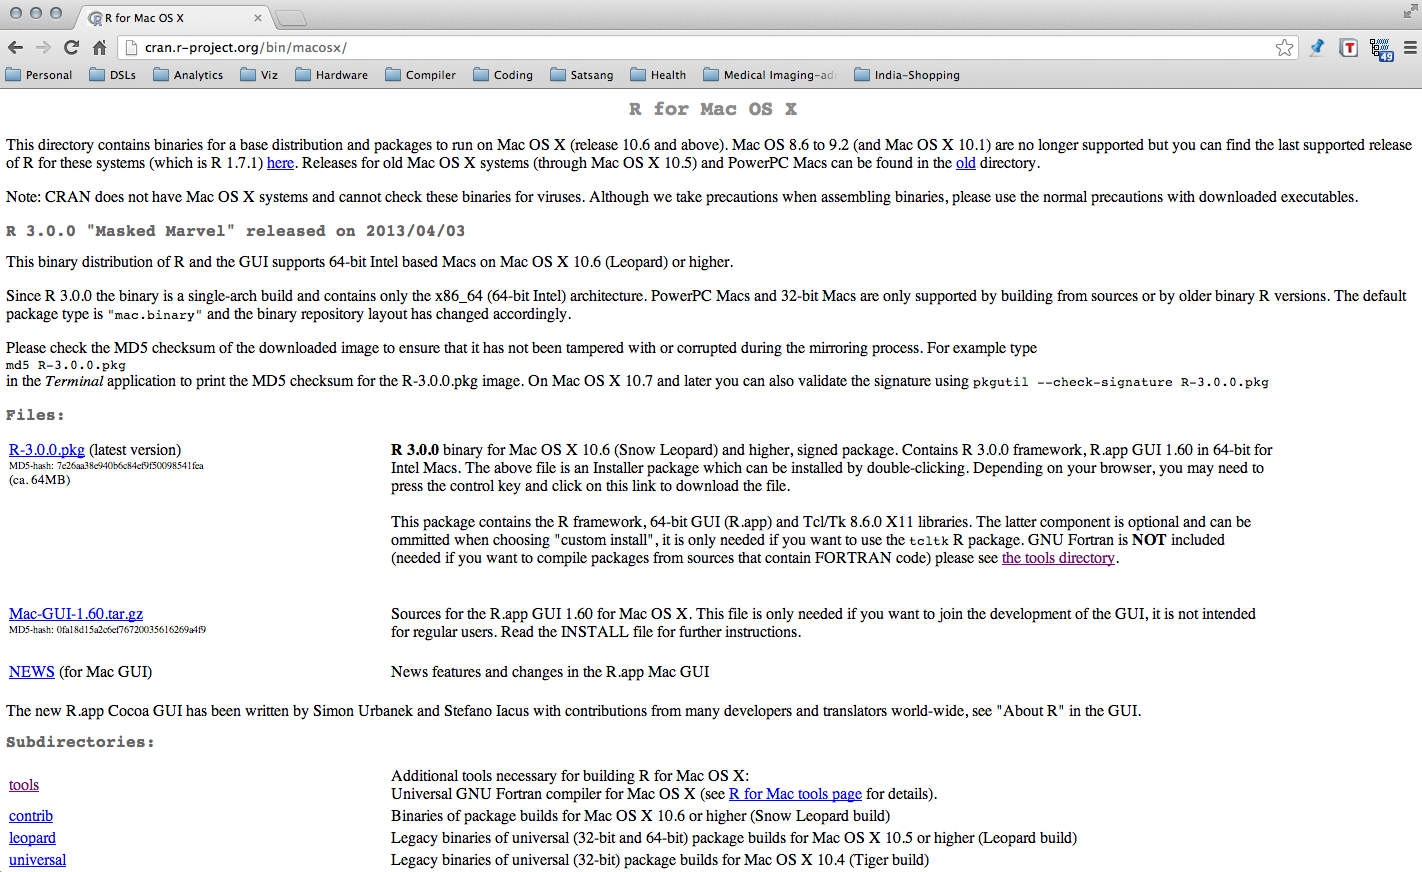
\includegraphics[scale=.3]{mac/pics/R_Mac_1.png}\end{center}}
  %
  Download the \proglang{R} dmg package for Mac OS X.  We recommend grabbing the latest version of \proglang{R} available.
  \sshots{\begin{center}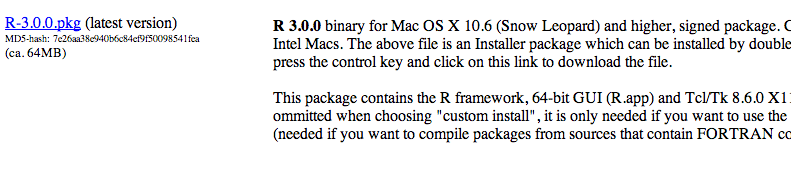
\includegraphics[scale=.7]{mac/pics/R_Mac_2_2.png}\end{center}}
  %
  \item Open the saved file from \ref{enum:macdl} above to begin the installation.  At the first setup screen, click 'Continue' to begin the installation process.
  \sshotm{mac/pics/R_Mac_3.png}
  %
  \item At the 'Read Me' section, read the important information and then click 'Continue'.
  \sshotm{mac/pics/R_Mac_4.png}
    %
  \item When prompted with the software license agreement, you must click 'Agree' to proceed.  \proglang{R} is distributed under a free, ``copyleft'' license (GPL v3).  You can read the license by clicking 'Read License'.  Once you agree to the terms, click 'Agree'.
  \sshotm{mac/pics/R_Mac_5.png}
    %
  \item From the 'Installation Type' section, we recommend you use the defaults.  However, you may change the install location by selecting 'Change Install Location\dots'.  Once you have made your choice, click 'Install'.
  \sshotm{mac/pics/R_Mac_6.png}
    %
  \item Next, you will be prompted for your computer's name and password.  Enter the appropriate information and click 'Install Software' to begin the installation process.
  \sshotm{mac/pics/R_Mac_7.png}
  %
  \item Once the installation process begins, wait a few moments for the packages to validate and install.
  \sshotm{mac/pics/R_Mac_8.png}
  %
  \sshotm{mac/pics/R_Mac_9.png}
  %
  \sshotm{mac/pics/R_Mac_10.png}
  %
  \sshotm{mac/pics/R_Mac_11.png}
  %
  \item Once the installation completes successfully, click 'Close' to finish the installation process.
  \sshotm{mac/pics/R_Mac_12.png}
  %
\end{enumerate}

Out of the box, you can run an interactive \proglang{R} session in two separate ways:  from the ``gui'' and from a terminal.  To launch the \proglang{R} ``gui'', simply go to your Applications folder in Finder and double-click \code{R.app}.
  \sshots{\begin{center}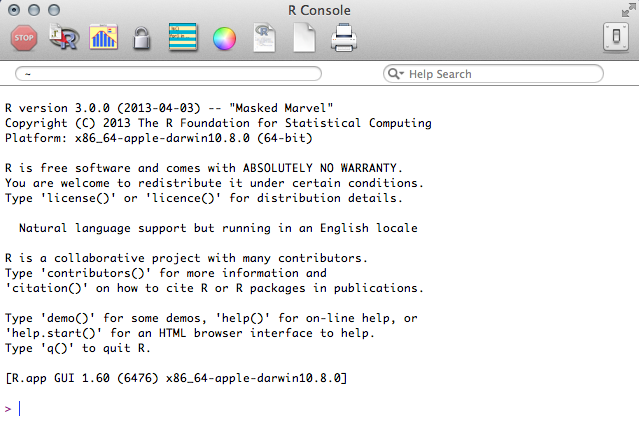
\includegraphics[scale=.8]{mac/pics/R_Mac_13.png}\end{center}}

Once \proglang{R} is finished installing, you need to install the  \href{http://cran.r-project.org/web/packages/rlecuyer/index.html}{\pkg{rlecuyer}} package.  To install it from an interactive \proglang{R} session, simply start an \proglang{R} session and issue the command
\begin{lstlisting}[language=rr]
install.packages("rlecuyer")
\end{lstlisting}





\subsubsection{Compiling from Source}

You can find \proglang{R} sources from \url{http://cran.r-project.org/sources.html}

Start by opening a terminal and navigate to the folder containing the \proglang{R} source package you just downloaded.  You can extract the archive by executing, for example
\begin{lstlisting}[language=sh]
tar zxvf R-3.0.0.tar.gz
\end{lstlisting}

From here, generally it should be enough to simply execute
\begin{lstlisting}[language=sh]
./configure && make && make install
\end{lstlisting}
without problems.









\subsection{Installing MPI}

You have several options for installing OpenMPI on a Mac.  You can install from \href{https://www.macports.org/}{MacPorts}, which is a relatively simple way to manage compiling/installing of many packages (such as OpenMPI).  You can also compile from source.

Before beginning, make sure you have some ``downtime'' allotted, as the compilation will take upwards of a few hours for some machines.

\subsubsection{Installing from a MacPorts}

Arguably the easiest way to install OpenMPI for a Mac (that I'm aware of) is using \href{https://www.macports.org/}{MacPorts}, which is not unlike some source repositories for Linux.  You can find information about installing MacPorts from \href{https://www.macports.org/install.php}{MacPorts installation page}, maintained by the MacPorts project.

Once you have MacPorts installed, you can install openmpi from a terminal by issuing the command:
\begin{lstlisting}[language=sh]
sudo port install openmpi
\end{lstlisting}





\subsubsection{Compiling from Source}

If you want to install OpenMPI from source (I don't really recommend this unless you think you have a good reason to), then the sources are available \href{http://www.open-mpi.org/software/ompi/v1.6/}{here}.





\subsection{Installing pbdR Packages}
Installing pbdR should go smoothly.  The simplest way to install the packages is from an \proglang{R} terminal, which will manage dependencies for you much like the Mac App store.


\subsubsection{Installing from CRAN}
This is perhaps the simplest way to proceed, as \proglang{R} will handle any package dependency resolution for you.  Simply start an \proglang{R} session (from the terminal\footnote{Do \emph{not} use the gui.  See section~\ref{sec:porblam} for details}, type \code{R} then press enter) and issue the command:
\begin{lstlisting}[language=rr]
install.packages(<package>)
\end{lstlisting}
So for example, to install \pkg{pbdMPI}, you might execute:
\begin{lstlisting}[language=rr]
install.packages(pbdMPI)
\end{lstlisting}


\subsubsection{Installing from the Shell}
If you have downloaded a pbdR (or other \proglang{R}) package, then installing from the shell simply amounts to issuing the command:
\begin{lstlisting}[language=sh]
R CMD INSTALL <package>
\end{lstlisting}
So for example, to install \pkg{pbdMPI}, you might execute:
\begin{lstlisting}[language=sh]
R CMD INSTALL pbdMPI_0.1-6.tar.gz
\end{lstlisting}


\subsubsection{Installing from Github}
CRAN policy is such that updates to packages can not be made too frequently.  For this reason, the development versions of our packages will have bugfixes and new features much more quickly than CRAN versions.  

The easiest way to install from github is using Hadley Wichkam's \pkg{devtools} package (which can be installed via \code{install.packages(devtools)}).  Assuming you have this package installed, then from an \proglang{R} session, to install a pbdR package you would issue one of the following:

\begin{lstlisting}[language=rr]
library(devtools)

install_github(repo="pbdMPI", username="RBigData")
install_github(repo="pbdSLAP", username="RBigData")
install_github(repo="pbdNCDF4", username="RBigData")
install_github(repo="pbdBASE", username="RBigData")
install_github(repo="pbdDMAT", username="RBigData")
install_github(repo="pbdDEMO", username="RBigData")
\end{lstlisting}

You can also install \emph{really} new package builds, which will be very current in terms of features, but also bugs (or even complete package breakage).  If you're sure you want these packages, then you can install them as follows:

\begin{lstlisting}[language=rr]
# dev repo 1
install_github(repo="pbdMPI", username="snoweye")
install_github(repo="pbdSLAP", username="snoweye")
install_github(repo="pbdNCDF4", username="snoweye")
# dev repo 2
install_github(repo="pbdBASE", username="wrathematics")
install_github(repo="pbdDMAT", username="wrathematics")
install_github(repo="pbdDEMO", username="wrathematics")
\end{lstlisting}
